%!TEX root = ../tezisfuzet.tex
% ************************** Thesis Abstract *****************************

\section*{A téma ismertetése}

Az utóbbi néhány év kísérleti és számítógépes szimulációs vizsgálatai eredményeképpen kiderült, hogy a szubmikron méretű kristályos rendszerek deformációs tulajdonságai alapvetően eltérnek a tömbi anyagoknál megszokott viselkedéstől. Ebben a mérettartományban a deformációt diszlokációk kollektív mozgásával megvalósuló véletlen lavinák jellemzik\cite{Dimiduk1188}. Ezért a deformációs tulajdonságok leírására csak statisztikus módszerek használhatók. A doktori munka célja az egyelőre szinte teljesen ismeretlen statisztikus tulajdonságok kísérleti feltárása, valamint a jelenségek számítógépes szimulációval való jobb megismerése. Tekintve, hogy a nanotechnológia előretörésével az ipar mind gyakrabban használ olyan anyagokat, amelyek viselkedését alapvetően már e jelenségek dominálják, az elért eredmények közvetlen mérnöki alkalmazhatósága is jelentős.

\section*{Előzmények és célkitűzés}
\markboth{Előzmények és célkitűzés}{Numerikus modellek}
\subsection*{Numerikus modellek}

A munka első részeként célom a mikron méretű mintákban lejátszódó folyamatok statisztikus tulajdonságait (úgymint feszültség-deformációs görbe, leggyengébb-láncszem modellel való összevetés, diszlokációmintázat-képződés) tanulmányozni új modellek segítségével.

A diszlokációlavinák tekintetében ismert, hogy azok nemcsak számításigényesebb diszkrét diszlokációdinamikai (DDD) szimulációkkal modellezhetőek \cite{PhysRevLett.112.235501}, hanem magasabb skálájú, a diszlokációk kontinuum modelljére alapuló mezoszkopikus modellekkel is \cite{1742-5468-2005-08-P08004}. Egy ilyen modellben megjelenő szabad paramétereket kalibrálhatjuk az alacsonyabb szintű DDD szimulációk eredményei alapján. Így egy effektív modell kapható, amely mutatja a hasonlóságot az alacsonyabb szintű modellel az ahhoz illesztett paraméterekhez tartozó tulajdonságokban. Egy ilyen modell előnye a nagyobb hatékonysága, ami abban mutatkozik meg, hogy azonos számítógépes erőforrás és futtatási idő mellett nagyobb rendszerek is tanulmányozhatóak. Ehhez a fentiek értelmében az kell, hogy létezzenek olyan, a makroszkopikus szerkezetben mérhető és definiálható mennyiségek, amelyek leírják az effektív modell skálája alatt, a mikroszerkezetben végbemenő folyamatokat. Egy ilyen modell különösképp előremutató, ha a hasonló viselkedés az illesztett tulajdonságokon túl másban is megmutatkozik, és ha a használhatósága túlmutat az eredeti modell alkalmazhatóságán.

\begin{enumerate}
\setcounter{enumi}{0}
\item Célom, hogy egy új, a diszlokációk kontinuumelméletén alapuló mezoszkopikus modellt dolgozzak ki, amelynek a szabad paramétereit úgy választom meg, hogy az a legjobban közelítse a vizsgált tulajdonságokban az alacsonyabb skálájú DDD modellek eredményét.
\end{enumerate}

Már a diszlokációk első megfigyelése óta tudható, hogy azok az anyagban nem homogén módon helyezkednek el, hanem mintázatokba rendeződnek. Ez a mikroszerkezet fontos következménnyel jár a makroszkopikus viselkedésben, ugyanis pl. ilyen diszlokációszerkezetek okozzák a ciklikus deformáció során megjelenő állandósult csúszási sávokat, ami az anyag kifáradásához és repedéséhez, végül töréséhez vezet. Ezek a szerkezetek abban is szerepet játszanak, hogy a különböző, mikron méretű mikrooszlopok – ún. mikropillárok -- deformációs válaszai lényegesen eltérnek egymástól. Az ezen szerkezeteket leíró modellek többsége fenomenológikus megközelítésű, és míg egyesek olyan paramétereket tartalmaznak, amelyek mikroszkopikus eredete nem megmagyarázott, mások olyan viselkedéseket jósolnak, amelyeket kísérletileg nem figyeltek meg. Éppen ezért jelent nagy előrelépést egy olyan modell, ami pusztán a DDD modellből kiindulva felépíti a diszlokációk kontinuumelméletét -- amelynek minden paramétere a mikroszerkezet által meghatározott --, és lehetővé teszi a diszlokációmintázatok tanulmányozását. A mintázatok kialakulásának lehetőségét a modellen elvégzett lineáris stabilitáselemzés mutatja, ami összekapcsolja a modell makroszkopikus paramétereit a mintázat tulajdonságaival, például a jellemző hullámhossz nagyságával \cite{PhysRevB.93.214110}. Noha a kialakuló teljes mintázatról, annak robosztusságáról analitikusan kevés állítható, a matematikai modell numerikus implementációival ezek vizsgálhatóvá válnak.

\begin{enumerate}
\setcounter{enumi}{1}
\item Célom, hogy egy új, a diszlokációk kontinuumelméletén alapuló mezoszkopikus modellt dolgozzak ki, amely számot ad a diszlokációmintázat-kialakulásról a lineáris stabilitáselemzés tartományán kívül, és lehetővé teszi a mintázatok robosztusságának vizsgálatát.
\end{enumerate}

\subsection*{Kísérlet}
\markboth{Előzmények és célkitűzés}{Kísérlet}
A kísérleti vizsgálatok eddig gyakorlatilag csak néhány mikron átmérőjű mikropillárok nanoindenterrel való összenyomásával történtek. Ennek nagy hátránya, hogy a pillár FIB-bel történő kimunkálása és az összenyomás más berendezésben történt, ami nem teszi lehetővé, hogy in situ módon kövessük a lavinák következtében kialakuló felületi lépcsők megjelenését. Egy olyan méretű nanoindenterrel azonban, amely mintával együtt elfér a pásztázó elektronmikroszkóp vákuumkamrájában, lehetőség nyílik in situ deformációs kísérletek elvégzésére.

A deformációs kísérletek során számos adat gyűjthető a bekövetkező szerkezetváltozásról az akusztikus jelek érzékelésével. Azonban a különféle végbemenő folyamatok és az azok keltette jelek összepárosítása nem egyértelmű feladat, mert a jelek javarésze -- tömbi minta esetén -- a minta belsejéből származik, és a változás csak mikroszkopikus skálán látható. Egy, a mikropillárhoz csatolt akusztikus emissziós detektorral azonban, ha az összenyomást in situ követjük, összetársíthatjuk a folyamatokat a detektált jellel, különös tekintettel a diszlokációlavinákra. Ezzel lehetőség nyílik teljesen új, az irodalomban eddig nem ismert mérések elvégzésére is. 

\begin{enumerate}
\setcounter{enumi}{2}
\item Célom egy olyan nanoindenter kifejlesztése, amivel megvalósítható egy olyan mérési összeállítás, amelyben mikropillárok deformációját pásztázó elektronmikroszkópban in situ módon követhetjük, miközben a mintához csatolt akusztikus detektorral a diszlokációlavinák keltette akusztikus jeleket detektáljuk.
\end{enumerate}.

Tekintettel arra, hogy a szimulációval vizsgálható rendszerek mérete ugyan abba a nagyságrendbe esik, mint a kísérletileg tanulmányozható mintaméret, a két módszerrel kapott eredmények közvetlenül összehasonlíthatók. Ez unikális lehetőséget teremt a szubmikronos plaszticitás tulajdonságainak jobb megértésére.

\section*{Alkalmazott módszerek}
\markboth{Alkalmazott módszerek}{Numerikus modellek}
\subsection*{Numerikus modellek}

\Citet{1742-5468-2005-08-P08004} munkája nyomán egy sejtautomata (angolul cellular automaton, CA) modellt alkottam és programoztam meg. Ebben a modellben az anyag különálló részekből álló egységek (cellák) sokaságából áll, amik egymással csak az azok plasztikus deformációja során fellépő feszültségeken keresztül hatnak kölcsön. A CA modellben a cellaszintű folyáshatárt ($\tau_w$-t) valószínűségi változóként kezelve azt úgy kalibráltam, hogy az első, legkisebb külső feszültség mellett megjelenő lavinánál a külső feszültség eloszlása ugyanaz a Weibull-eloszlás legyen, mint ami az alacsonyabb DDD szimulációkban látható. A $\tau_w$ várható értékét és a cellákban alkalmazott diszkrét deformációs lépés nagyságát úgy kalibráltam, hogy a feszültség-deformációs görbe két másik, különböző fajta DDD modellek görbéi közé essen. A $\tau_w$ valószínűségi változó mivolta miatt a rendszer deformációs válasza minden rendszerre más és más, és adott rendszerre is nemdeterminisztikus a fejlődése. A kívánt paraméterek összehasonlításához ezért nagymennyiségű szimulációs eredményt kell elemezni.

Egy ilyen CA modell alkalmas lehet olyan belső rendezetlenséggel rendelkező, alakítási lágyulást szenvedő anyagok törésének modellezésére is, ahol a törést a deformáció lokalizáció okozza. Ehhez bevezettem a modellben egy lágyulási mechanizmust. Az így kapott modellben a rendszer rendezetlenségét a $\tau_w$ eloszlása biztosítja. Ez a belső rendezetlenség nem szükségszerűen a diszlokációk rendezetlenségét mutatja, mi több, a vizsgált anyagnak még csak kristályosnak sem kell lennie. A vizsgált anyag lehet fémüveg, fémhab, vagy bármilyen, a fenti feltételeknek megfelelő anyag, amely egy magasabb skálán már homogén módon kezelhető.

A diszlokációmintázatok tanulmányozására egy olyan CA modellt dolgoztam ki, amely a fenti modell mozgásegyenleteiben található feszültségtagokon túl további olyanokat is tartalmaz, amelyeket a kontinuumelmélet lokálissűrűség-közelítése segítségével a diszlokációk korrelációjából eredeteztethetőek. Egy ilyen modellben ugyancsak nagy szerepe van a véletlen folyamatoknak, amely jelentkezik egyrészt a különböző kezdeti folyáshatár-eloszlásban, másrészt nemdeterminisztikus időfejlődésben. Ezen sztochasztikus folyamatok eredményeként a fejlődő mintázatok részleteikben rendszerről rendszerre mások, azonban több szimulációs eredményt együttesen kiértékelve a közös tulajdonságaik megállapíthatók. A mintázat jellemző hullámhosszát az egyes rendszerek diszlokációsűrűségéből úgy határozhatjuk meg, hogy azokat Fourier-térben átlagoljuk. A rendszer robosztusságát a sztochasztikus folyamatok erősségének állításával és extremális dinamika alkalmazásával vizsgálhatom. Utóbbi alatt azt értem, hogy feltételezem, hogy csak azon diszlokációk mozognak, amelyekre a legnagyobb erők hatnak.

\subsection*{Kísérlet}
\markboth{Alkalmazott módszerek}{Kísérlet}
Kereskedelmi forgalomban kapható eszközök segítségével elmozdulást már nanométeres tartományban mérhetünk kapacitív szenzorok segítségével, valamint tárgyakat is mozgathatunk speciális lineáris motorok segítségével. A minta feszültség-deformáció görbéjét megadhatjuk a benyomófej elmozdulása, illetve a benyomófejre ható erő segítségével. Ezen értékek kimérésének a biztosításához egy három részből álló nanoindenter-testet terveztem az \ref{fig:rugo} szerint. A keret $d$ elmozdulása egy lineáris motor segítségével előírható az állványhoz képest. A benyomófej kerethez képesti $e$ elmozdulását pedig egy kapacitív szenzor méri. Ezen adatokból kiszámolható a minta alakváltozása, $\epsilon = d - e $, másrészt a rugó összenyomódása, ami szintén $\epsilon$. Utóbbiból a nanoindenter benyomófejére ható erő -- a rugó erő - rugalmas deformáció görbéjének ismeretében -- kiszámolható.

\renewcommand{\figurename}{Ábra.}
\begin{figure}[htbp!] 
\centering    
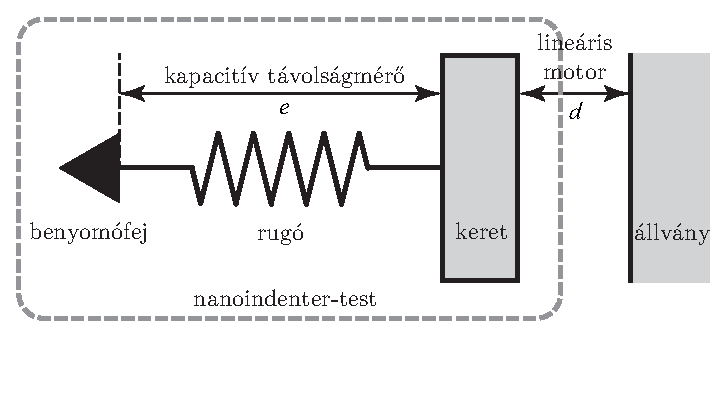
\includegraphics[width=1\textwidth]{rugo}
\caption{A nanoindenter-test vázlatos szerkezete. A rugók egyedi kialakítása lehetővé teszi, hogy a benyomófej csak az összenyomás tengelyében mozdul el. A kerethez képesti elmozdulását nagypontosságú kapacitív elmozdulásmérővel mérjük. A keret az állványhoz képest egy lineáris motorral mozgatható nanométeres pontossággal.}
\label{fig:rugo}
\end{figure}

Ehhez a nanoindenter-testet egytömb alumíniumból terveztem meg, amelyben a rugókat számos lamellából álló lap, mintegy egymás mögé hajtogatott laprugók biztosítják. A szikraforgácsolás kellően precíz és finom megmunkálásnak bizonyult, hogy egy ilyen törékeny elrendezést meg lehessen valósítani. Egy ilyen elrendezés képes a nyomás irányában \si{\micro\newton} pontossággal erőt mérni, de az erőmérés közben a deformációs tengely irányától eltérő irányba nem mozdul el, máskülönben a $d$ távolságot nem lehetne kellő pontossággal mérni.

A vákuumkamrában a rugó csillapodását nem biztosítja a levegő közegellenállása, ezért a rugó és benyomófej tartója alá helyezett állandó mágnessel örvényáramok keltésével lehet azt elérni.

\section*{Tézispontok}
\markboth{Tézispontok}{ }
\begin{enumerate}
\item Megmutattam, hogy kristályos anyagok felbonthatóak olyan egységek rendszerére, amely egységek mérete a diszlokációk korrelációs hosszánál nagyobb, és az ilyen rendszerek vizsgálhatóak hatékonyan sejtautomaták segítségével. A kis deformációs tartományának vizsgálatával fel lehet úgy paraméterezni egy ilyen modellt, hogy az hasonló viselkedést mutasson a diszkrét diszlokációdinamikai szimulációkkal. Ez a hasonlóság megmutatkozik az első lavinákhoz tartozó külső feszültség eloszlásában, annak szórásában és a rendszermérettel való skálázódásában, továbbá a feszültség-deformációs görbe alakjában. Egy ilyen rendszer skálázási tulajdonságait két független exponens határozza meg. Az egyik az első lavinához tartozó külső feszültség eloszlásának exponense, a másik pedig meghatározható az azonos deformációhoz tartozó külső feszültség szórásából. \cite{PhysRevB.95.054108}

\item Megmutattam, hogy olyan, belső rendezetlenséggel rendelkező, de nagyskálán homogén anyagok, amelyek alakítási lágyulást szenvednek, és törésük a deformáció lokalizációjára vezethető vissza, hatékonyan modellezhetőek sejtautomata modellekkel. Megmutattam, hogy a belső rendezetlenség növelése eredményeként, noha a képlékeny alakváltozás már kisebb feszültségeknél elkezdődik, a törésig alkalmazható maximális erő és az elérhető képlékeny alakváltozás nagysága megnő. \cite{Tuzes2017}

\item A diszlokációk kontinuum-elmélet leírásában elegendő a lokálistér-sűrűség közelítésig felírni a mozgásegyenlet tagjait ahhoz, hogy az így kapott rendszerben mintázatképződést figyeljünk meg. Megmutattam, hogy ezek mozgásegyenleteit megoldhatjuk egy sejtautomata rendszerrel sztochasztikus tagok jelenléte mellett és a kifejlődött mintázatok összhangban vannak az eredeti mozgásegyenleteken alkalmazott lineáris stabilitáselemzési jóslattal. \cite{PhysRevB.98.054110}

\item Új nanoindentációs eszköz testét terveztem meg és kiviteleztem, amelynek segítségével lehetővé vált pásztázó elektronmikoszkópban mikroméretű oszlopok deformációjának in situ vizsgálata, és a berendezéshez csatolható akusztikus emissziós detektor segítségével összepárosíthatóvá váltak a pásztázó elektronmikroszkópban megfigyelt folyamatok és a detektált akusztikus jelek. A nanoindenter rugójának újszerű kialakítása lehetővé teszi a benyomófej kerethez képesti elmozdulásának pontos mérését kapacitív távolságmérő segítségével, ezáltal meghatározhatóvá téve a benyomófejre ható erő is. \cite{hegyi}
\end{enumerate}

\section*{Kitekintések, további lehetőségek}
\begin{itemize}
\item Lehetőség van a 2-es tézispontban említett modell paramétereit alacsonyabb skálás, molekuladinamikai szimulációk segítségével felparaméterezni, így a modell jóslatait konkrét anyagokra lehet vonatkoztatni.

\item Az 1-es és 3-as pontban említett sejtautomata modellek egyesíthetőek, és a várakozás szerint egy ilyen modell egyesítené a két modell alkalmazhatósági területét. Egy ilyen modell különösképp előremutató volna, ha kiderülne, hogy alkalmazhatósága ennél szélesebb körű.

\item A 4-es pontban említett nanoindentációs eszköz célja, hogy nagymennyiségű adatot lehessen gyűjteni számos mikrooszlop összenyomásáról. Ez egy jelenleg is futó kutatás a kutatócsoportban. A legnagyobb mérési hibát, zajt vagy mérési nehézséget okozó alkatrész további fejlesztésével a mérések még értékesebbé válhatnak. Lehetőség van például a rugók és a benyomófej közti rész tömegének jelentős csökkentésére, ami a mikrooszlopok deformációjának gyorsabb és pontosabb lekövetését tenné lehetővé.
\end{itemize}